\documentclass{article}
\usepackage[T1]{fontenc}
\usepackage{lmodern}
\usepackage{graphicx}
\usepackage{amsmath,amssymb}
\usepackage[a4paper,margin=2cm]{geometry}
\usepackage[absolute,overlay]{textpos}
\setlength{\TPHorizModule}{1mm}
\setlength{\TPVertModule}{1mm}
\usepackage[indonesian]{babel}
\usepackage{hyperref}
\setlength{\emergencystretch}{2em}
% unit: Halaman 19

\begin{document}

% === Halaman 19 (llm) ===

\vspace{236.12mm}

Contoh hasil file cipherteks: hasil.enc

% deskripsi: Screenshot aplikasi Notepad yang menampilkan isi file 'hasil.enc' yang berisi teks acak hasil enkripsi (cipherteks).
% bbox normalisasi: [0.0640, 0.1250, 0.7720, 0.9200]
\begin{textblock*}{148.68mm}(13.44mm,37.12mm)
\noindent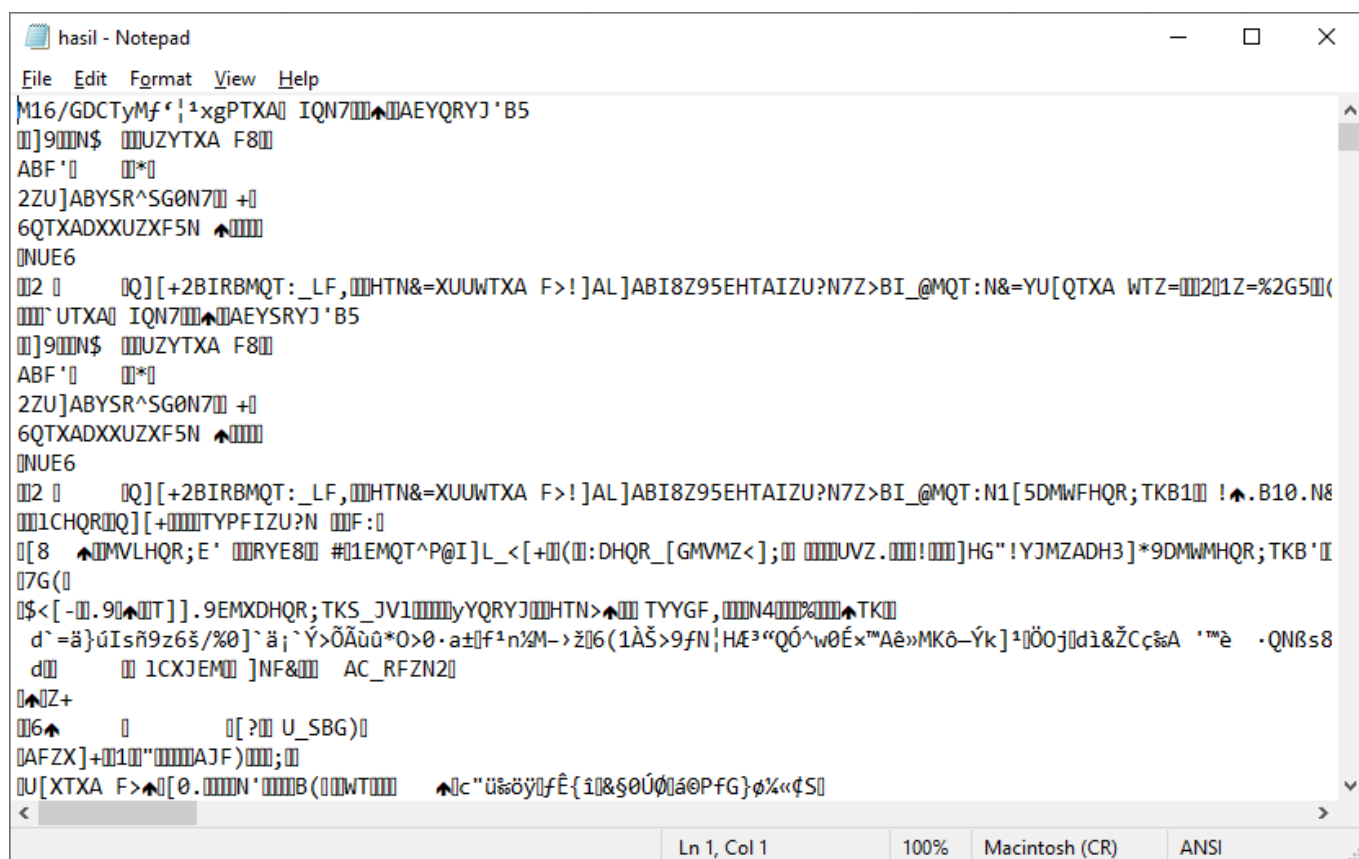
\includegraphics[width=148.68mm,height=236.12mm]{../../images/llm/page_019_img_01.png}%
\end{textblock*}

\end{document}
